\documentclass[10pt,usenames,dvipsnames]{beamer}
\usetheme[progressbar=foot, block=fill]{metropolis}

\usepackage[utf8]{inputenc}
%\usepackage[T1]{fontenc}
\usepackage{amsmath}
\usepackage{amsfonts}
\usepackage{amssymb}
\usepackage{graphicx}
%\usepackage[MeX]{polski}
\usepackage{fancybox}
\usepackage[normalem]{ulem}
\usepackage{ucs}
\usepackage{tikz}
\usepackage{pgfplots}
\usepackage{listings}
\usepackage{fancyvrb}
\usepackage{setspace}
\usepackage{silence}
\usepackage{booktabs}
\usetikzlibrary{shapes,arrows, positioning, calc, fit}
\WarningFilter{latex}{Overwriting}
\WarningFilter{latexfont}{LaTeX Font Warning}
\WarningFilter{latex}{LaTeX Font Warning}
\WarningFilter{latexfont}{Font shape}
\WarningFilter{latexfont}{Some font}
\WarningFilter{latexfont}{Size substitutions}
\tikzset{
  invisible/.style={opacity=0},
  visible on/.style={alt={#1{}{invisible}}},
  alt/.code args={<#1>#2#3}{%
    \alt<#1>{\pgfkeysalso{#2}}{\pgfkeysalso{#3}} % \pgfkeysalso doesn't change the path
  },
}
\pgfplotsset{compat=1.10}
\title{PartSeg}
\subtitle{Image analysis tool}
\author{Grzegorz Bokota}
\institute{Center of New Technologies, Uniwersity of Warsaw} 
\begin{document}
\maketitle
\begin{frame}[c]{Agenda}
  \tableofcontents%[allsubsections]
\end{frame}
\section{Algorithm}
\subsection{Segmentation algorithm}
\begin{frame}[c]{Basic Flowchart of segmentation process}
  \begin{center}
    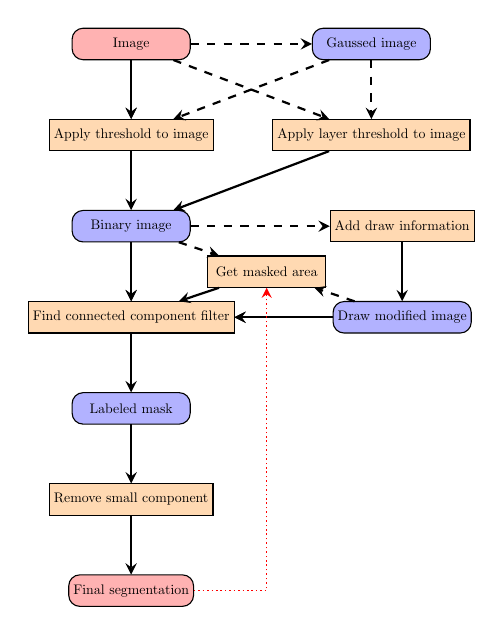
\begin{tikzpicture}[scale=0.5, node distance=1.5cm, transform shape]
      \tikzstyle{startstop} = [rectangle, rounded corners, minimum width=3cm, minimum height=.8cm,text centered, draw=black, fill=red!30]
      \tikzstyle{data} = [rectangle, rounded corners, minimum width=3cm, minimum height=.8cm,text centered, draw=black, fill=blue!30]
      \tikzstyle{process} = [rectangle, minimum width=3cm, minimum height=.8cm, text centered, draw=black, fill=orange!30]
      \tikzstyle{decision} = [diamond, minimum width=3cm, aspect=4, text centered, draw=black, fill=green!30]
      \tikzstyle{arrow} = [thick,->,>=stealth]
      \node (image) [startstop] {Image};
      \node (threshold) [process, below=of image] {Apply threshold to image};
      \node (layerthreshold) [process, right=of threshold, visible on=<3->] {Apply layer threshold to image};
      \node (gaussimage) [data, above=of layerthreshold, visible on=<2->] {Gaussed image};
      \node (binmask) [data, below=of threshold] {Binary image}; 
      \node (conn) [process, below=of binmask] {Find connected component filter};
      \node (bindraw) [data, right=of conn, visible on=<4->, xshift=1cm] {Draw modified image}; 
      \node (draw) [process, above=of bindraw, visible on=<4->] {Add draw information};
      \node (labeledmask) [data, below=of conn] {Labeled mask};
      \node (filter) [process, below=of labeledmask] {Remove small component};
      \node (final) [startstop, below=of filter] {Final segmentation};
      \node (mask) [process, visible on=<5->] at ($(conn)!0.5!(draw)$) {Get masked area};      
      \draw [arrow, visible on=<1>] (image) -- (threshold);
      \draw [arrow, visible on=<2->, dashed] (image) -- (threshold);
      \draw [arrow, visible on=<2->, dashed] (image) -- (gaussimage);
      \draw [arrow, visible on=<3->, dashed] (image) -- (layerthreshold);
      \draw [arrow, visible on=<2->, dashed] (gaussimage) -- (threshold);
      \draw [arrow, visible on=<3->, dashed] (gaussimage) -- (layerthreshold);
      \draw [arrow] (threshold) -- (binmask);
      \draw [arrow, visible on=<3->] (layerthreshold) -- (binmask);
      \draw [arrow, visible on=<1-3>] (binmask) -- (conn); 
      \draw [arrow, visible on=<4->, dashed] (binmask) -- (conn);
      \draw [arrow, visible on=<4->, dashed] (binmask) -- (draw);
      \draw [arrow, visible on=<4->] (draw) -- (bindraw);
      \draw [arrow, visible on=<4>] (bindraw) -- (conn);
      \draw [arrow, visible on=<5->, dashed] (bindraw) -- (conn);
      \draw [arrow, visible on=<5->, dashed] (bindraw) -- (mask);
      \draw [arrow, visible on=<5->, dashed] (binmask) -- (mask);
      \draw [arrow, visible on=<5->] (mask) -- (conn);
      \draw [arrow] (conn) -- (labeledmask);
      \draw [arrow] (labeledmask) -- (filter);
      \draw [arrow] (filter) -- (final);
      \draw [arrow, semithick, densely dotted, red, visible on=<5>] (final) -| (mask);
 

    \end{tikzpicture}
  \end{center}
\end{frame}
\begin{frame}[c]{Summarize}
  \begin{itemize}
    \item To maximize speed algorithm remember intermediate steps
    \item<2-> \textbf{But this is memory consuming}
    \item<2-> This allow to not rerun algorithm from scratch 
    \item<3-> Can use segmentation result as mask in next iteration 
    \item <3-> Mask can be dilated by given radius
  \end{itemize}
\end{frame}
\begin{frame}[standout]{}
  This is tool for \emph{small} files  
\end{frame}
\subsection{*.cmap files create algorithm}
\begin{frame}[c]{cmap create – flowchart}
  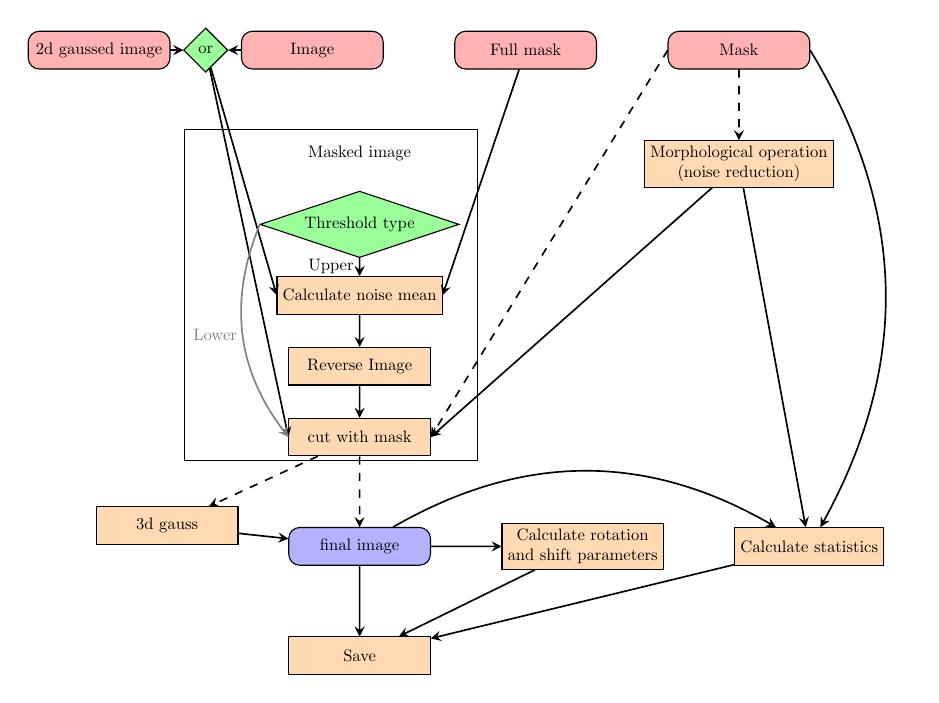
\begin{tikzpicture}[scale=0.6, node distance=1.5cm, transform shape]
    \tikzstyle{startstop} = [rectangle, rounded corners, minimum width=3cm, minimum height=.8cm,text centered, draw=black, fill=red!30]
    \tikzstyle{data} = [rectangle, rounded corners, minimum width=3cm, minimum height=.8cm,text centered, draw=black, fill=blue!30]
    \tikzstyle{process} = [rectangle, minimum width=3cm, minimum height=.8cm, text centered, draw=black, fill=orange!30]
    \tikzstyle{decision} = [diamond, aspect=1, text centered, draw=black, fill=green!40]
    \tikzstyle{arrow} = [semithick,->,>=stealth]
    \node (image) [startstop] {Image};
    \node (fullmask) [startstop, right=of image] {Full mask};
    \node (mask) [startstop, right=of fullmask] {Mask};
    \node (gaussimage) [startstop, left=of image] {2d gaussed image};
    \node (morph) [process, below=of mask, align=center] {Morphological operation\\(noise reduction)};
    \node (orimg) [decision] at ($(image)!.5!(gaussimage)$) {or};
    \node (maskedimg) [below=of image, xshift=1cm ] {Masked image}; 
    \node (trtype) [decision, aspect=3, below of=maskedimg] {Threshold type}; 
    \node (noisemean) [process, below of=trtype] {Calculate noise mean};
    \node (reverse) [process, below of=noisemean] {Reverse Image}; 
    \node (cutimg) [process, below of=reverse] {cut with mask};
    \node (gaus3d) [process, below left=of cutimg] {3d gauss}; 
    \node (finalimg) [data, below=of cutimg] {final image};
    \node (save) [process, below=of finalimg] {Save};
    \node (center) [process, right=of finalimg, align=center] {Calculate rotation\\and shift parameters};
    \node (statistics) [process, right=of center] {Calculate statistics};
    \node [draw=black, minimum height=7cm, minimum width=6.2cm, xshift=-0.6cm] at ($(maskedimg)!.5!(cutimg)$) {};
    \draw [arrow] (gaussimage) -- (orimg);
    \draw [arrow] (image) -- (orimg);
    \draw [arrow] (fullmask) -- (noisemean.east);
    \draw [arrow, dashed] (mask.west) -- (cutimg.east);
    \draw [arrow, dashed] (mask) -- (morph);
    \draw [arrow] (morph) -- (cutimg.east);
    \draw [arrow] (orimg) -- (noisemean.west);
    \draw [arrow] (orimg) -- (cutimg.west);
    \draw [arrow] (trtype) -- node[left] {Upper} (noisemean);
    \draw [arrow] (noisemean) -- (reverse);
    \draw [arrow, gray] (trtype.west) to [bend right] node[left]{Lower} (cutimg.west);
    \draw [arrow] (reverse) -- (cutimg);
    \draw [arrow, dashed] (cutimg) -- (gaus3d);
    \draw [arrow, dashed] (cutimg) -- (finalimg);
    \draw [arrow] (gaus3d) -- (finalimg);
    \draw [arrow] (finalimg) -- (center);
    \draw [arrow] (finalimg) to [bend left] (statistics);
    \draw [arrow] (finalimg) -- (save);
    \draw [arrow] (center) -- (save);
    \draw [arrow] (statistics) -- (save);
    \draw [arrow] (mask.east) to [bend left] (statistics);
    \draw [arrow] (morph) -- (statistics);
  \end{tikzpicture}
\end{frame}

\section{User interface}
\begin{frame}[c]{Overview}
  \begin{figure}[htpb]
    \centering
    \includegraphics[width=1\linewidth]{interface}
    \caption{Program interface}
    \label{fig:name}
  \end{figure}
\end{frame}
\begin{frame}[c]{Summarize}
  \begin{enumerate}
    \item \textbf{This is beta version} – still need tests.
    \item In project files there are saved information about every step needed to get segmentation. 
    \item Program allow to save set of profiles.
    \item Program allow to change segmentation to mask. 
    \item I think tat every useful, in segmentation, information are showed on main window.
    \item Project specific settings are in Advanced Window.
    \item Statistics are in Advanced Windows.
    \item files from previous version demand change extension form \texttt{.gz} to \texttt{.bz2}.
  \end{enumerate}  
\end{frame}
\begin{frame}[standout]{}
  This is tool for \emph{small} files  
\end{frame}
\begin{frame}[c]{Plans}
  If they are useful and I have time.  
  \begin{enumerate}
    \item Add more statistics and allow user to choose which should be calculated.
    \item Add automatic and multi files processing based on profiles (need discussion).
    \item Pack PartSeg to executable. 
  \end{enumerate}  
\end{frame}
\begin{frame}
  \begin{center}
    \Huge Thank for Your attention
  \end{center}
\end{frame}
\end{document}
